\documentclass{standalone}
\usepackage{tikz,amsmath,graphicx,calc,chemfig}
\usepackage[update,verbose=false]{epstopdf}
\usepackage[version=3]{mhchem}
\graphicspath{{./figs/}}
\usetikzlibrary{
    arrows,
    decorations.pathmorphing,
    backgrounds,
    positioning,
    fit,
    petri
}
\setatomsep{1.4em}
\setbondoffset{.1em}
%\setcrambond{.3em}{1pt}{.0em}
\renewcommand*\printatom[1]{{\ensuremath{\mathsf{#1}}}}


\begin{document}
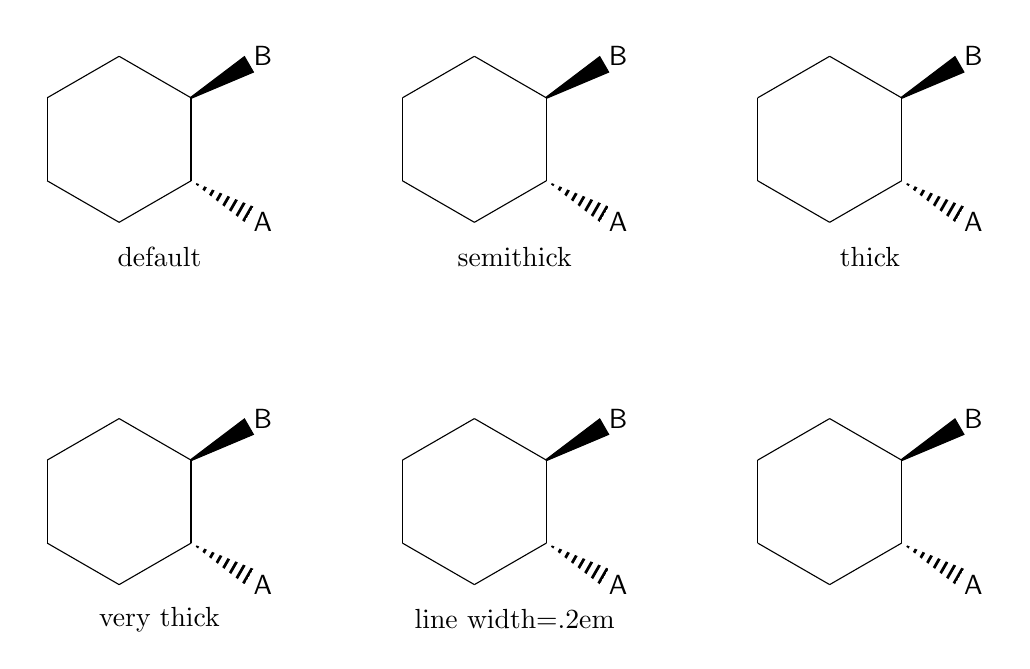
\begin{tikzpicture}
    [scale=1,
     structure/.style={rectangle,draw=white,fill=white,
               outer xsep=.2cm,outer ysep=.2cm,minimum size=2mm,node distance=0.4cm},
     label/.style={rectangle,fill=white,font=\bfseries,
               outer ysep=.2cm,minimum size=4mm,},
     arrow/.style={->,>=stealth',semithick},
     reagent/.style={text width=2cm,font=\footnotesize,align=center,midway},
     designbox/.style={rectangle,draw=black,thick,fill=red,
               inner sep=0pt,minimum width=15mm, minimum height=2.5mm, node distance=0mm},
               line join=rounded]
    %
    \matrix[column sep=1.4cm,row sep=2cm]{
        \node[structure] (chexane) {\chemfig{*6(--(<:A)-(<B)---)}}; &

        \setbondstyle{semithick}
        \node[structure] (chexane2) {\chemfig{*6(--(<:A)-(<B)---)}}; &

        \setbondstyle{thick}
        \node[structure] (chexane3) {\chemfig{*6(--(<:A)-(<B)---)}}; \\

        \setbondstyle{very thick}
        \node[structure] (chexane4) {\chemfig{*6(--(<:A)-(<B)---)}}; &

        \setbondstyle{line width=.2em}
        \node[structure] (chexane5) {\chemfig{*6(--(<:A)-(<B)---)}}; &

        \setbondstyle{semithick}
        \setcrambond{.3em}{1pt}{.0em}
        \node[structure] (chexane6) {\chemfig{*6(--(<:A)-(<B)---)}}; \\
    };

    \draw (chexane.south)  node{default};
    \draw (chexane2.south) node{semithick};
    \draw (chexane3.south) node{thick};
    \draw (chexane4.south) node{very thick};
    \draw (chexane5.south) node{line width=.2em};
%    \draw (chexane6.south) node{semithick with different cram bond style};
\end{tikzpicture}
\end{document}
